\subsection{Compartmentalization}
%objective
I estimated the degree of compartmentalization calculating the relative area or volume of expression of genes during development.
My intention here was not to focus on individual genes, but to get a global overview of the embryo compartmentalization and differentiation processes based on expression data of thousands of genes, i.e., using a statistical approach.

One would expect, and it has been implicitly assumed \citep{Carroll2001} \citep{Davidson2001} that the compartmentalization of the embryo (as I measure it here) increases during development.
However, the specific temporal dynamics of this increase in any species is not known. Neither is clear if the dynamics should be similar for different species, or for different groups of genes.
As the development of \textit{Ciona} and \textit{Drosophila} are very different and it would be impossible to compare them stage-by-stage, I focused here in three major developmental periods: pre-gastrula, gastrula, and post-gastrula stages. These periods are easily recognizable in both species facilitating the comparative analysis.

%results
I found that in both species, the relative area or volume decreased in a non-linear way (see Figs X). 
However, the timing of the major decrease was different.
In \textit{Drosophila} the major decrease occurred at very early development, from maternal to early gastrula stage (Fig. \ref{fig:Art-I-3measures}).
Practically half of the genes in follows this decrease pattern: 46\% of the genes were characterized as having a non-linear decrease in their relative area.
In contrast, in \textit{Ciona} the volume of expression decreases mostly after gastrulation (between the 112-cell and the early tailbud stage).
However less dramatic, I found significant differences between the 32-cell and 64-cell stages, and between the 64-cell and 112-cell stages.

\begin{figure}[h]
  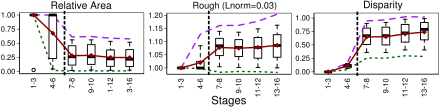
\includegraphics[width=\textwidth]{./Images/Art-I/3_measures.png}
  \centering
  \caption{Distribution plot of the relative area of expression (left), roughness (center) and disparity (right) for all genes in each stage. Diamonds represent the mean, boxes the IQR. Whiskers 10 and 90 percentiles. Dashed line represents the max values and dotted line the min values (mean of the last and first decile, respectively). Stages on the x-axis, vertical dashed line represents gastrulation entry.}
  \label{fig:Art-I-3measures}
\end{figure}

% discussion
The difference in the timing of the major change on compartmentalization between species must relate to differences in their specific development.

The earlier compartmentalization of \textit{Drosophila} is most probably due to its derived early development, namely, the syncytial blastoderm. 
During the blastoderm stage, approximately 4,000 cell nuclei can `communicate' with each other only by TFs \citep{Jaeger2011}. The direct cross regulation of gene expression facilitates a rapid and highly dynamic process which seems to be responsible for the early spatial restriction of a great proportion of developmental genes.

In contrast,  \textit{Ciona}'s early embryonic patterning is based on maternal determinants and signalling events mostly between neighbouring cells \citep{Lemaire2009}, which act in a combinatorial way \citep{Hudson2007} to establish a unique TF combination in more than half of the blastomere pairs before gastrulation \citep{Imai2006} determining most of their fates.
Thus, even when in \textit{Ciona} most of the cell fates are already determined (by the specific combination of a fraction of TFs) and the embryo can be said to be already highly compartmentalized, this is not evident at the global level of gene expression, which I am measuring here.


Therefore, the `delay' of compartmentalization observed in \textit{Ciona} could be explained by the relatively slower process of signal transduction (as in \textit{Ciona}) compared to the gap gene network (in \textit{Drosophila}).

%%%%%%%%%%%%%%%%%%%%%%%%%%%%%%%%%%%%%%%%%%%%%%%%%%%%%%%%%%%%%%%%%%%%%%%%%%%%%%%%%%%%%
\subsection{Disparity}
%objective
As the relative area (or volume) of expression informs on how genes are expressed in progressively smaller regions in the embryo, the disparity can inform about how different regions of the embryo express increasingly different combinations of genes.

Therefore, both measures reflect slightly different aspects of complexity that are independent from each other. A decrease in the volume of expression of genes does not necessarily imply an increase in spatial disparity: genes could decrease their volume of expression but end up restricted to the same parts of the embryo. 
If the majority of genes would be expressed ubiquitously (this is large volume), however, then the mean disparity between its regions would be necessarily low. 

%results
My results show that in each species, the global disparity pattern is similar to the relative area or volume patterns.
Therefore, in Drosophila the disparity increases mostly in the transition from the maternal to early gastrula and in Ciona this major change occurs after gastrulation.

FIGURA CIONA 3 MEDIDAS

% discussion
It is important to notice that these measures should not necessarily correlate, as it could be that between two stages the relative area of expression decreases but not the disparity if the genes are expressed in the same part of the embryo or vice-versa.

In \textit{Ciona} I found an example of such case, when there is no perfect correspondence between the relative volume and the disparity of expression: disparity increased significantly between early to mid-tailbud stages but no significant differences between the relative volume of expression of these stages were found (II, Fig. 3A).

This means that, on average, genes are expressed in a similar number of tissues in these stages, but in the mid tailbud the combination of genes expressed in these tissues are more different between each other. This shows that the disparity measure is complementary to the relative volume measure to describe the compartmentalization of the embryo.


%%%%%%%%%%%%%%%%%%%%%%%%%%%%%%%%%%%%%%%%%%%%%%%%%%%%%%%%%%%%%%%%%%%%%%%%%%%%%%%%%%%%% 
\subsection{2D and 3D roughness analyses}




%%%%%%%%%%%%%%%%%%%%%%%%%%%%%%%%%%%%%%%%%%%%%%%%%%%%%%%%%%%%%%%%%%%%%%%%%%%%%%%%%%%%% 
\subsection{Synexpression territories}
